% !TEX root = deckblatt2b.tex

\section{RL-Hochpass}

\begin{figure}[H]
  \begin{center}
    %\tikzset{component/.style={draw,thick,circle,fill=white,minimum size =0.75cm,inner sep=0pt}}
    \begin{circuitikz}
      \draw (0,2)
      to[R=$R$] (3,2)
      to[short] (6,2);
      \draw (4,2)
      to[L=$L$] (4,0);
      \draw (0,0)
      to[short] (6,0);
      \draw (0,1.8)
       to[short] (0,0.7) node[vee] {};
      \draw (-0.5,1) node[] {$U_e$};
      \draw (6,1.8)
       to[short] (6,0.7) node[vee] {};
      \draw (6.5,1) node[] {$U_a$};
    \end{circuitikz}
    \caption{RL-Hochpass 1.Ordnung}
    \vspace{1cm}
    Das Schaltbild zeigt den Messaufbau des RL-Hochpassfilters 1.Ordnung. \\
    $R=47\Omega, L=1mH, U_e=1V$\\
  \end{center}
\end{figure}

\subsection{Sprungantwort}
\begin{figure}[H]
 \begin{center}
  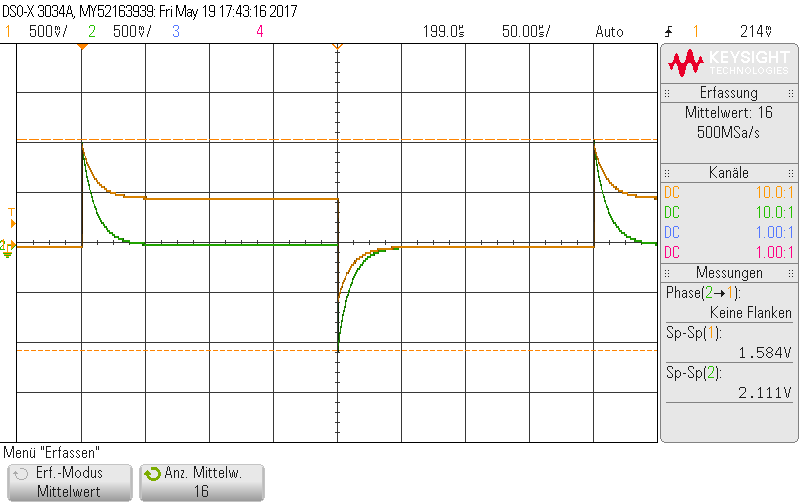
\includegraphics[height=6cm,width=12cm]{Oszi_Bilder/RL_Sprung}
 \end{center}
 \caption{Sprungantwort RL-Hochpass}
\end{figure}
\noindent
In der Abbildung der Sprungantwort sind die Aus- und Einschaltvorgänge an der Spule zu sehen. \\
\begin{align*}
 U_{charge} &= U_e e^{-\frac{t}{\tau}}\\
 U_{drain} &= -U_e e^{-\frac{t}{\tau}}\\
 \tau &= \frac{L}{R}\\
\end{align*}
\noindent
In der Abbildung beträgt die Eingangsspannung weniger als $0,5V$, da der Frequenzgenerator eine Spannungsquelle ist und den durch die Spule verursachten Stromfluss
nicht genügen kann. Die Induktivität der Spule ist auch verantwortlich für die Ausschläge beim Einschalten der Eingangsspannung. \\
Die Zeitkonstante kann aus der Sprungantwort abgelesen werden, indem man die Zeitdifferenz von $U_e=0$ bis $U_L \approx 0,3U_e$ misst. Daraus ergibt
sich ein $\tau_{gemessen}$ von $23\mu s$, dass gegenüber einem $\tau_{berechnet}$ von $21,28\mu s$ steht. Der Messfehler entsteht dabei, durch ungenauigkeiten
beim Ablesen mit dem Cursor und Bauteiltoleranzen.\\

\subsection{Bode Diagramm}

Das Bode Diagramm zeigt den Verlauf der Dämpfung und des Phasenwinkels des Filters in abhängigkeit der Frequenz.\\
\begin{figure}[H]
  \centering
  \begin{tikzpicture}
    \begin{axis}[width=15cm, height=7cm, xmode=log, xmin=10, xmax=1e7, xlabel={$Hz$}, ylabel={dB},y tick label style={grid=major}]
      \addplot table[x=Frequenz, y=dB, col sep=comma] {csv_files/RL_dB.csv};
      \node[label={340:{$f_g$}},square,fill=blue,inner sep=3pt] at (axis cs:7480.28,-3) {};
    \end{axis}
  \end{tikzpicture}
  \caption{Bode Diagramm RL-Hochpass, Dämpfung}
\end{figure}
\noindent
Die niedrigen Frequenzen werden vom Hochpassfilter stark gedämpft. Die Dämpfung nimmt bei steigender Frequenz, mit $20dB/DEK$, ab. Ist die Grenzfrequenz, von 
$f_g = \frac{R}{2\pi L} = 7480,28Hz$ erreicht, wird das Signal ungedämpft durchgelassen. Der Knick bei $50Hz$ ensteht durch den Spannungsteiler, der sich durch den
parasitären Innenwiderstand der realen Spule ergibt. Dieser wird mit zunehmender Frequenz von der steigenden Impedanz der Spule überdeckt.\\

\begin{figure}[H]
  \centering
  \begin{tikzpicture}
    \begin{axis}[width=15cm, height=7cm, xmode=log, xmin=10, xmax=1e7, xlabel={$Hz$}, ylabel={$\phi$},y tick label style={grid=major}]
      \addplot table[x=Frequenz, y=Phi, col sep=comma] {csv_files/RL_Phi.csv};
      \node[label={0:{$f_g$}},square,fill=blue,inner sep=3pt] at (axis cs:7200,45) {};
    \end{axis}
  \end{tikzpicture}
  \caption{Bode Diagramm RL-Hochpass, Phasengang}
\end{figure}
\noindent
Der Phasengang verläuft von $0^\circ$ bis $70^\circ$ und nimmt dann wieder ab. Die Spule besitzt, auf Grund ihres Innenwiderstandes, zwei Phasenlagen von jeweils $45^\circ$, 
jedoch entspricht nur die um $7500Hz$ der Grenzfrequenz.\\
\\
Durch den, vom Spulenstrom verursachten, Spannungseinbruch des Frequenzgenerators wurde die Messung des Frequenzganges nicht beeinträchtigt, da hierbei lediglich
das Verhältnis der Ausgangs- zur Eingangsspannung betrachtet wird. Die Messergebnisse stimmen auch weitestgehend mit der Simulation der realen Spule, mit parasitären 
Innenwiderstand, überein. \\